\documentclass[10pt,a4paper]{article}
\usepackage[margin=2.3cm]{geometry}
\usepackage[T1]{fontenc}
\usepackage[utf8]{inputenc}
\usepackage{lmodern}
\usepackage{microtype}
\usepackage{amsmath,amssymb}
\usepackage{booktabs}
\usepackage{graphicx}
\usepackage{xcolor}
\usepackage[hidelinks]{hyperref}
\usepackage{url}
\usepackage{enumitem}
\setlist{nosep}

\newcommand{\pfree}{p_{\mathrm{free}}}
\newcommand{\EM}{\mathrm{EM}}

\title{ENGRAFT: writing a hundred facts into the n-gram memory table\\
of a mixture-of-experts language model by gradient descent on a usage corpus}
\author{fulvian\\\small \texttt{fulviold@gmail.com} \quad
\url{https://github.com/fulvian/engraft-ngram}\\\small \url{https://engraft-engram.dev}}
\date{2026-09-26 \quad (technical report, version 3)}

\begin{document}
\maketitle

\begin{center}
\fbox{\parbox{0.92\textwidth}{\small
\textbf{How this was built.} The code, the experiments and this write-up were
produced in Claude Code sessions (Anthropic's Claude) driven by a
single human operator who set the goals, approved every design step, ran the
hardware and read every result. Design, implementation, adversarial review and
independent verification were done by separate model instances; the human made
the calls. We say this up front because we think you should know it before reading
the numbers. We are not after stars: we want the method checked, broken and improved.}}
\end{center}

\begin{center}
\fbox{\parbox{0.92\textwidth}{\small
\textbf{What changed in version 3 (2026-09-26).} The report is brought level with
release \texttt{v0.2.2} of the repository: an English cell and a direct test of whether a
fact crosses languages (Section~\ref{sec:lang}); a rerun of the composition probes without
the protocol confounds of the first run (Section~\ref{sec:results}); a statement of what the
method is and is not (Section~\ref{sec:idea}); and the cost stated without the timings of the
unreleased execution path.

\smallskip
\textbf{Since version 1 (2026-09-05).} Version 1 described the
\emph{surgical graft}: the eight trigram rows read by one trigger, optimized until the
answer token came out. Its measurements stand and its run of record reproduces at the
repository tag \texttt{v0.1.0}; Section~\ref{sec:v1} summarizes them and states why the
method was abandoned. This version describes what replaced it, \emph{usage-corpus
descent}: a plain language-model loss on a corpus of sentences that use the facts,
descended over a budgeted set of the table rows that corpus reads, with the mixture-of-experts routing
first captured from the base model and then released. It reports results on a corpus of
one hundred facts, measured on the real inference engine against a test set frozen before
the descent, and the failure mode that dominates the residual. The engineering that turns
the principle into a pipeline (turning documents into a usage corpus, choosing the row
budget, calibrating the two tuning constants, and the optimized execution path)
is not part of this report; the descent, the measurements, the corpus, the overlays and the
result files are released with it.}}
\end{center}

\begin{abstract}
Some recent language models carry an explicit n-gram memory: at every position the last
two and three tokens are hashed into a small set of rows of a large lookup table, and the
rows are added to the residual stream at one early block (DeepSeek's \emph{Engram};
Qwen3.8-Flash-Next ships one with 16 heads). ENGRAFT writes facts into such a table after
training, without touching a weight: the edit is an overlay of table rows that the
inference engine substitutes at read time. The method applies to models with an
Engram-style table; every measurement here is on Qwen3.8-Flash-Next. Given a set of facts
and a corpus of short fragments that use them (statements, questions, cloze forms, chat
turns, paraphrases), we take as variables a budgeted set of the table rows those fragments
read, and minimize the negative log-probability of the answer tokens through a replica of
the frozen model, with each fact weighted by its training mass. No teacher is needed: a
control experiment on 24 facts ranks the answer first on 86 of 112 held-out fragments
against 50 for the same descent imitating the model with the fact document in its prompt,
and 0 for a negative control. The mixture-of-experts routing is held at the base model's
choices while the rows move most, then released so that the descent trains the computation
the engine will actually run; releasing it raises exact-match recall by 0.17--0.19. The
descent stops on the rate of improvement of held-out first-token accuracy. On a corpus of
one hundred invented facts in Italian, the real llama.cpp engine with the overlay
reproduces the full answer on 0.841 and 0.873 of 841 frozen test fragments for two seeds
(base model 0.005). The mean KL divergence from the base model on neutral text is
0.012--0.013 nats, about four times a quantization yardstick measured at 24 facts. The
residual failures are dominated by a contest between facts of the same subject, which
share the rows their triggers read; the overlay decodes to the fact with the larger
training mass, and weighting the loss by that mass reduces but does not remove the
effect. Preliminary Chinese and English cells score below Italian, and at equal training
mass per fact the Chinese and Italian cells are indistinguishable. A fact does not cross languages: the Italian test set run against the
Chinese overlay reproduces the base model's numbers exactly, although the engine reads the
overlay's rows.
\end{abstract}

\section{Problem and idea}
\label{sec:idea}

Adding a fact to a trained language model usually means fine-tuning, a parameter-efficient
adapter, a locate-and-edit rewrite of MLP weights \cite{rome,memit}, or leaving the fact in
the prompt (retrieval). All of these change or bypass computation that every input goes
through. Models built on DeepSeek's Engram design \cite{engram} offer a different handle:
an explicit, hash-addressed memory table whose rows are read only when an exact n-gram
occurs. If a fact can be written into the rows that its uses read, the edit is local by
construction: contexts that never produce those n-grams never read those rows, the
weights are untouched, and the edit can be removed by deleting a file.

The difficulty is that the rows do not act on the output directly. They enter the residual
stream through a learned gate that depends on the hidden state, at one early block, and
everything that follows (delta-net and attention layers, the remaining blocks of
mixture-of-experts routing) transforms them. A one-step write through the unembedding
\cite{userengram} steers the output projection directly; we instead differentiate through
the whole path, from the rows to the answer token.

The first form of the method (Section~\ref{sec:v1}) did this one trigger at a time: eight
rows, one answer. It worked on the trigger and on nothing else, because the rows are the
same when the fact is stated in a paragraph but the hidden state at the gate is not. The
current form (Section~\ref{sec:method}) takes the opposite stance: the fact is not a
trigger but a set of \emph{uses}, the variables are a budgeted set of the rows those uses read, and the
loss is the ordinary language-model loss on the answers across the uses. The n-gram table
then does what it was trained to do, store what a context should produce, for a corpus it
never saw.

\paragraph{What this is, and what it is not.} ENGRAFT is token-addressed memory written by
gradient descent. It is not general model editing, and it is not a replacement for retrieval.
A written fact lives in the rows its n-grams hash to: it acts when a prompt contains those
n-grams and is invisible otherwise, so it has to be written in the language, and largely in
the phrasings, in which it will be asked (Section~\ref{sec:lang} measures the language half).
In exchange the fact sits inside the model's own forward pass: it costs no context tokens,
needs no retriever, index or second model at inference, travels as one file next to the
model, and deleting the file restores the model bit for bit. It is not cheaper to store than
text: the overlay costs about 90\,KB per fact, while the training fragments behind it come to
749 tokens per fact.

\section{The n-gram table in Qwen3.8-Flash-Next}
\label{sec:mech}

Qwen3.8-Flash-Next (the \texttt{qwen4exp} architecture in llama.cpp \cite{pr27742}) has 48
blocks, 512 experts of which 10 are used per token, and a per-layer-embedding (PLE) table
of 16 heads with rows of 160 floats; the table holds $5.1\times10^{10}$ values, about
20 million rows per head, stored in the GGUF as IQ4\_NL (4-bit) blocks. At each position
$t$, with context $[x_t, x_{t-1}, x_{t-2}]$ (an end-of-sequence token cuts the context),
the engine computes a mixed hash of the bigram and of the trigram with the model's own
multipliers, and each of the 8 bigram heads and 8 trigram heads takes the hash modulo its
own row count as a local row index. The 16 rows are gathered, transformed (a per-head
normalization, a direct linear path and a short causal convolution path), gated per
residual stream by a sigmoid of a signed square-root inner product with the hidden state,
and added to the four hyper-connection streams of block~1. The repository's
\texttt{docs/mechanism.md} documents the addressing, and \texttt{engraft/table.py}
reproduces it offline from the GGUF alone; the engine fork's overlay path
(\texttt{engine/README.md}) substitutes rows listed in a \texttt{.pleo} file at gather
time.

Two facts about this mechanism drive the method. First, the key is exact: changing one
of the last three tokens changes the 8 trigram rows, and changing the last two changes all
16, so an edit is invisible to every context that does not produce the same token windows.
Second, the rows act only through the gate and the downstream blocks, so the useful
direction in row space is not a function of the rows alone: it has to be found by
differentiating through the model, under the routing the model will actually use.

\section{The first form, and why it was abandoned}
\label{sec:v1}

Version 1 of this report grafted one fact at a time. A fact was a trigger and an answer of
at most three tokens (\emph{Oliver Hale's dog is called} $\to$ \emph{Pumpkin}); the
variables were the 8 trigram rows read at the trigger's last position (Figure~\ref{fig:mech});
the loss was $-\log p(\text{answer})$ at that position, descended through a CPU replica of
the frozen model with the expert routing recomputed at every step; the descent stopped when
the answer's probability under free routing exceeded 0.95. On eight neutral facts, the
quantized engine put the answer's first token at rank~1 with probability 0.85--0.96 for
seven of them; merging the eight overlays changed no measurement to the last digit, since
the grafts touched disjoint rows; the replica agreed with the full-precision engine on
17 of 17 grafts to $3\times10^{-5}$ in probability. Wall time was 7--17 minutes per fact.

\begin{figure}[t]
\centering
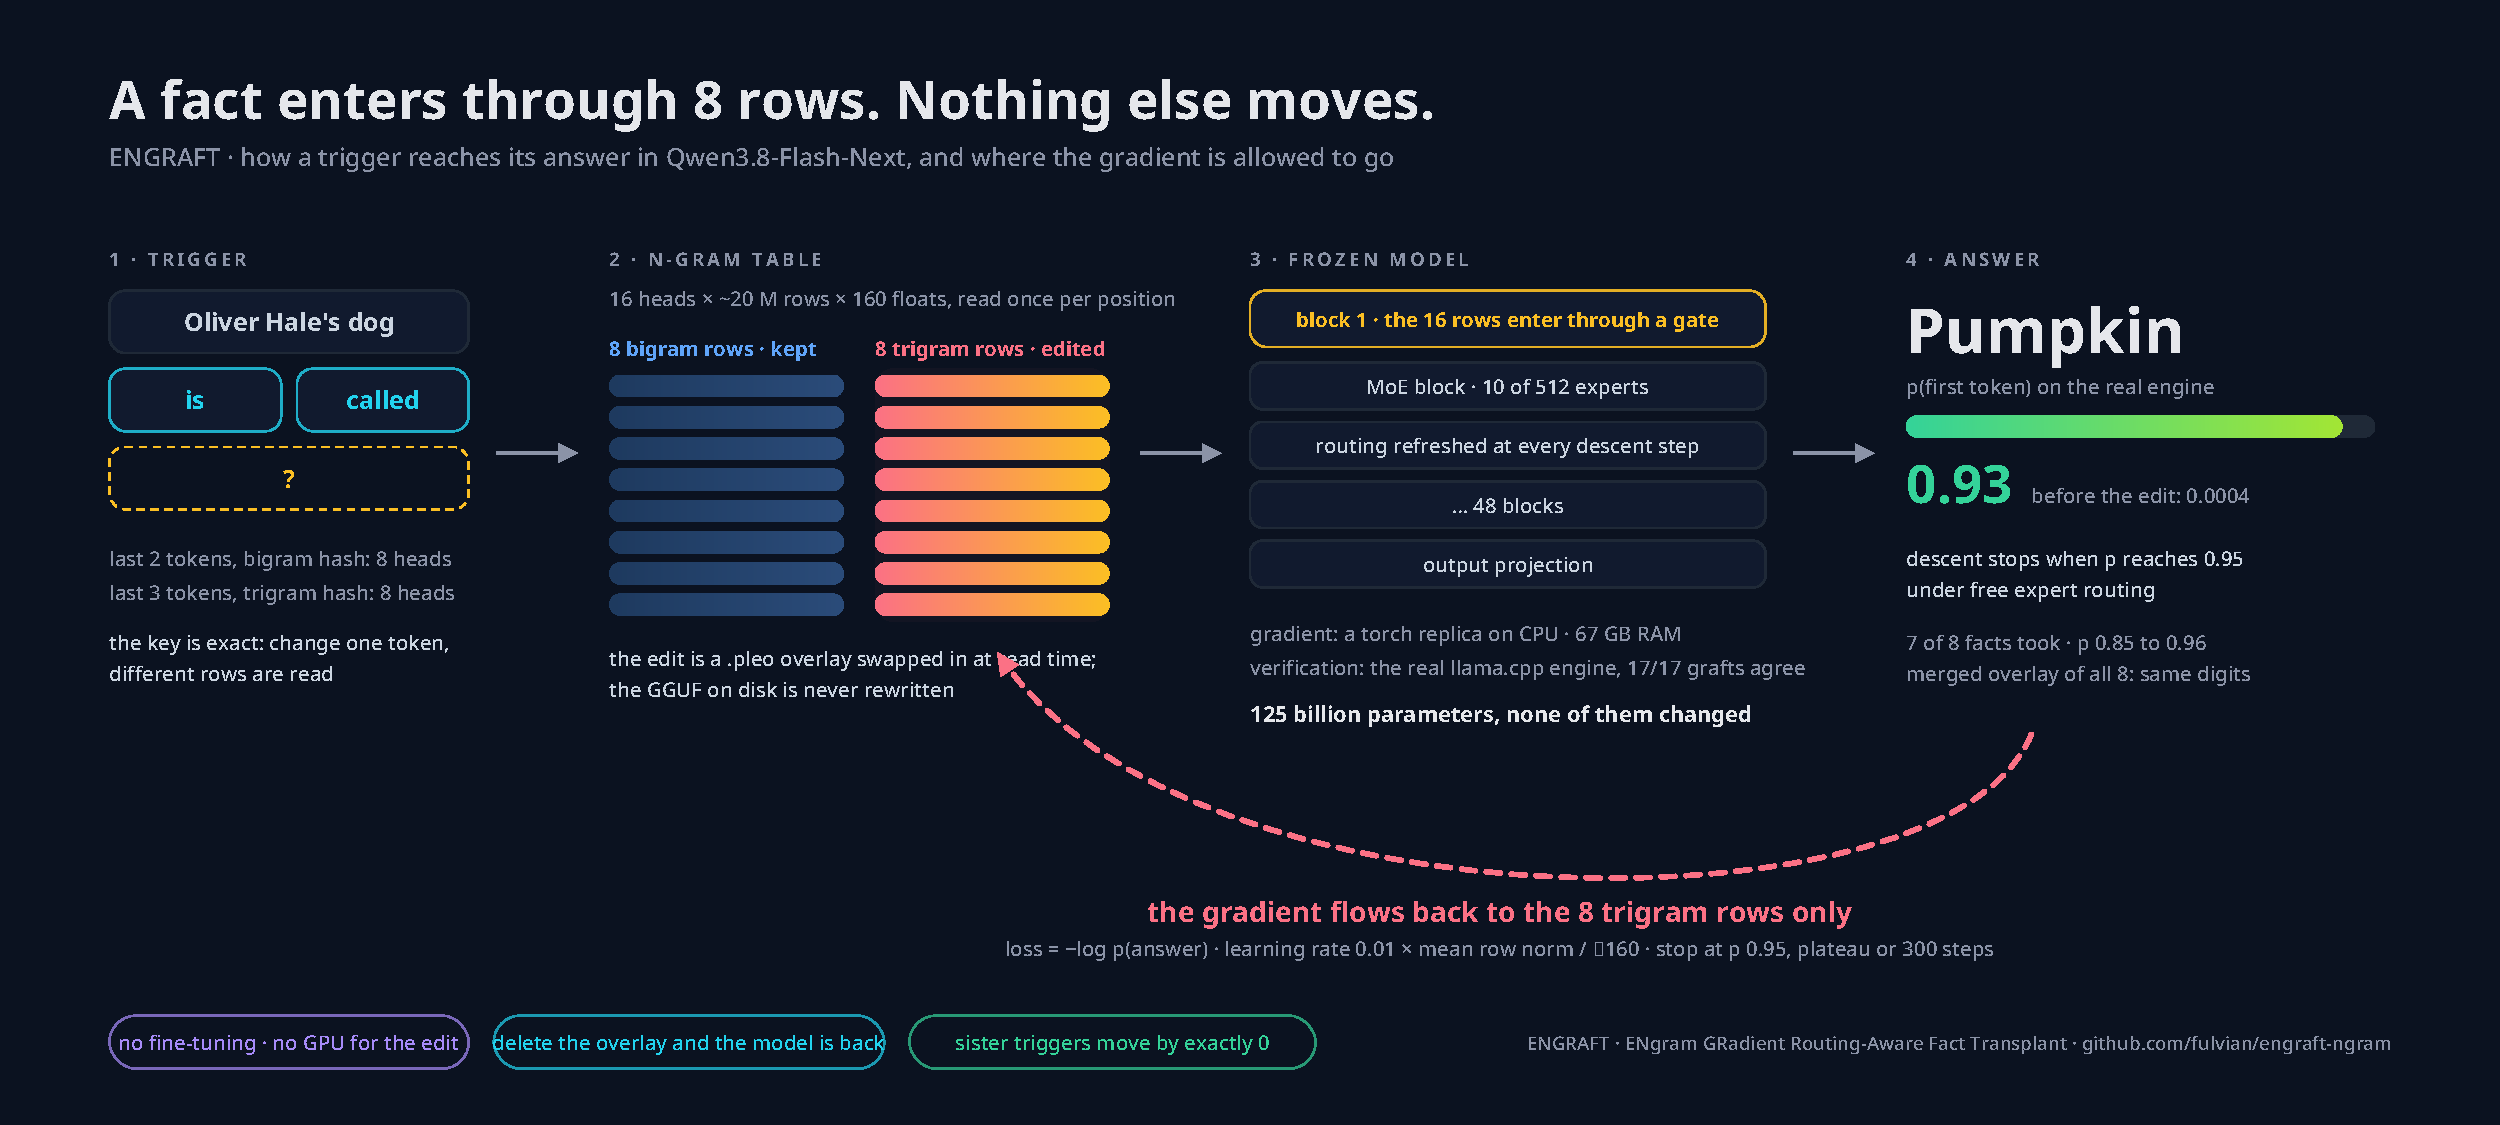
\includegraphics[width=\textwidth]{mechanism.pdf}
\caption{The mechanism, as used by the first form of the method: the trigger's last three
tokens are hashed into 16 rows of the table, 8 keyed by the bigram and 8 by the trigram;
the rows enter the frozen model at one early block; the loss is the answer's
log-probability at the output. The first form updated only the 8 trigram rows of one
trigger; the current form updates a budgeted set of the rows read by a corpus of uses. The result in both
cases is a \texttt{.pleo} overlay swapped in at read time; the GGUF is never rewritten.}
\label{fig:mech}
\end{figure}

It did not generalize. A same-tail paraphrase, which changes words before the trigger's
last three tokens and reads the very same 16 rows, put the answer at rank~1 for one fact
of eight; the fact stated verbatim inside a four-sentence document transferred for two of
six, although the grafted rows were read there. The rows were the same; the hidden state
at the gate was not, and with it the gate and everything downstream. One counterfactual
fact never took: the base model's next-token distribution at its trigger was concentrated
on a syntactic form, and eight rows at block~1 could not displace it. Version 1 reported
this as the main open problem. The answer was not a better trigger but a different
object: the fact as a distribution over its uses.

\section{Usage-corpus descent}
\label{sec:method}

\paragraph{The corpus.} A fact is a subject, a predicate and an answer. For each fact we
write short \emph{fragments} that use it, in several families: a statement that ends in
the answer, a question with its answer, a cloze form, a chat turn, a paraphrase; each
fragment carries the token span of its answer. The fragments are split into a
\emph{training} set, which the descent sees, a \emph{held-out} set of the same families,
which drives the stopping rule, and a \emph{test} set frozen before the first descent,
which is measured once, on the real engine, and never used for any decision. For the
corpus of Section~\ref{sec:results} these are 3\,209, 793 and 841 fragments for one
hundred facts.

\paragraph{The rows.} The variables are a set of table rows read by the corpus, chosen
within a row budget: for one hundred facts, 14\,032 rows out of $3.2\times10^{8}$, about 140
per fact. They are a subset of the 198\,628 rows that the training fragments read at all
positions; the budget, and the procedure that picks the rows within it, belong to the
pipeline and are not part of this report, but the resulting set is released with the
corpus. Nothing is chosen by hand. The rows stay in 32-bit floating point in an overlay;
the quantized table is never modified.

\paragraph{The loss.} The loss is the negative log-probability of the answer tokens at
their positions in each training fragment, summed over the fragments of a pack of
2\,048 tokens, plus the KL divergence from the base model's distribution at every other
position so that the rows do not learn to speak where they should be silent. The first
nine positions of each fragment are excluded, since the table has no useful context there.
A regularizer $\mu\,\lVert R - R_0\rVert^2/\lVert R_0\rVert^2$ keeps the variable rows $R$
near their original values $R_0$ ($\mu = 0.10$). The learning rate and $\mu$ are set once,
from a short calibration on the same corpus; there is no schedule.

\paragraph{Weighting by training mass.} Facts do not receive the same amount of training
text: the mass of a fact, counted as the number of loss positions its training fragments
contribute, ranges from 104 to 1\,426 on the corpus below (median 402).
Section~\ref{sec:contest} shows that this imbalance drives the dominant failure. The loss of
every fragment of fact $f$ is therefore multiplied by $w_f = \operatorname{median}(M)/M_f$,
where $M_f$ is the mass of $f$: light facts count more, heavy facts less, and the median fact
keeps weight one.

\paragraph{No teacher.} The method was first framed as context distillation: the same
model with the fact's source document in its prompt as teacher, the model with the overlay
as student. A control experiment on 24 facts and 112 held-out fragments, with everything
else identical, settled it: the plain language-model loss ranked the answer first on 86
fragments; imitating the teacher, on 50; a negative control with the answers replaced, on
0. The document in the prompt is a comparator for the ceiling, not a mechanism. The rest
of this report uses the plain loss.

\paragraph{Routing: captured, then released.} A mixture-of-experts model chooses ten of
512 experts per token at every block from the hidden state, and the rows change the hidden
state. Descending with the routing recomputed at every step (as version~1 did) makes
every regression coincide with a routing change; descending with the routing captured
once from the base model and held (\emph{routing-by-reference}) gives a smooth curve that
measures the wrong thing, since the engine will route freely. The descent therefore runs
in two phases. In the first, the routing at every block is the base model's, captured
once per fragment; the rows do the large movements against a fixed computation. When the
large movements are over (the growth of the overlay's norm has stalled and the rate of
improvement of held-out accuracy under captured routing has fallen well below its rate
under free routing, both for two consecutive readings), the routing is released and the
descent continues on the model's actual computation. On the corpus of
Section~\ref{sec:results} the release happens at step 140 of about 300; the free-routing
accuracy on the held-out set, which trailed the captured-routing accuracy during the first
phase, passes it within two readings after the release and finishes 0.03 above it.
Releasing the routing is what closes the gap between the replica's numbers and the
engine's: the same descent run entirely under captured routing loses 0.17--0.19 of
exact-match recall on the engine (Table~\ref{tab:cells}).

\paragraph{Stopping.} Every ten steps in the free phase (twenty in the captured phase)
the held-out fragments are scored under free routing, and the first-token accuracy $a_k$
is recorded. The descent stops when the local rate of improvement has fallen below a
fraction $\varphi$ of the total gain,
$L\cdot\text{slope}(a_{k-L+1},\dots,a_k)\,/\,(a_k - a_0) < \varphi$ with $L=4$ and
$\varphi=0.05$, for two consecutive readings. On the corpus below this fires between
steps 280 and 330. A hard cap is declared in advance: 320 steps in the captured-routing
cells, which the seed-0 cell reached one reading short of the criterion at the same
plateau as its sibling, and 480 in the released cells, never reached.

\paragraph{Verification on the engine.} The overlay is loaded into the llama.cpp fork and
measured on the frozen test set with greedy decoding: the answer's first token (rank and
probability) and \emph{exact match}, whether the greedy continuation reproduces the whole
answer. Collateral damage is measured as the KL divergence from the base model's
next-token distribution, under free routing, on sixteen random blocks of 2\,048 tokens of
neutral text (32\,768 positions) that contain none of the facts. A set of composition
probes asks for two facts in one answer. The replica's own free-routing first-token
accuracy is compared with the engine's on every test fragment.

\paragraph{Cost.} Every run was made on one workstation, an AMD Ryzen AI MAX+ 395 with
128\,GB of unified memory. One descent on one hundred facts runs 280--330 steps of one
2\,048-token pack each and takes hours; the engine measurements take hours more. The step is
bound by memory bandwidth. The measured runs used an optimized execution path for the expert
layers that is not released. The released reference path runs the same descent with
bit-identical expert logits; the compiled fusions of the optimized path change the loss by
about $2\times10^{-3}$, and a full rerun of the reference cell on the released path is
pending. The overlay for one hundred facts is a 9\,MB file, about 90\,KB per fact.

\section{Results on one hundred facts}
\label{sec:results}

\paragraph{The corpus.} One hundred facts about invented people and events, written in
Italian, stated in seven short documents of an invented world. The world is inspired, from
memory, by Philip K.~Dick's short story \emph{We Can Remember It for You Wholesale} (1966); no
text of the story was copied. 88 facts are invented outright and 12 follow the story as
remembered, unverified against the text; the base model turns out not to know them (it
answers 1 of their 89 test fragments without the overlay). One subject carries 32 of
the hundred facts, and one document states 60 of them. The fragments were written by a
large language model from the documents and validated automatically; the test set of
841 fragments (217 statements, 205 chat turns, 159 paraphrases, 134 questions, 126 cloze)
and 83 composition probes were frozen, with their hash recorded, before the first descent.
Without any overlay the engine reproduces 4 of the 841 answers (0.005) and puts the first
token at rank~1 for 0.095, inflated by numeric answers.

\begin{table}[h]
\centering\footnotesize
\setlength{\tabcolsep}{4pt}
\begin{tabular}{@{}llrrrrr@{}}
\toprule
cell & routing & steps & first token & exact match & exact match & KL to base \\
 & during descent & & rank 1 & (841 fragments) & (macro per fact) & (nats, mean) \\
\midrule
base & -- & -- & 0.095 & 0.005 & 0.004 & 0 \\
seed 0, captured & captured throughout & 320 & 0.702 & 0.625 & 0.646 & 0.0113 \\
seed 1, captured & captured throughout & 281 & 0.736 & 0.668 & 0.681 & 0.0115 \\
seed 0, released & captured to 140, then free & 301 & 0.842 & 0.823 & 0.837 & 0.0110 \\
seed 1, released & captured to 140, then free & 291 & 0.860 & 0.838 & 0.847 & 0.0103 \\
seed 0, mass-weighted & captured to 140, then free & 321 & 0.860 & 0.841 & 0.853 & 0.0131 \\
seed 1, mass-weighted & captured to 160, then free & 331 & 0.891 & 0.873 & 0.878 & 0.0116 \\
\bottomrule
\end{tabular}
\caption{Six descents on the same corpus, rows and hyper-parameters, measured on the real
quantized engine with greedy decoding on the frozen test set. \emph{Seed} changes the
order of the fragments in the packs; the released cells replay their captured cell exactly
up to step 140; the mass-weighted cells differ from the released ones only in the loss
weights (Section~\ref{sec:method}). KL: mean over 32\,768 positions of neutral text, free
routing. The two mass-weighted cells are released with the repository
(\texttt{data/quail/results/s0b}, \texttt{s1b}).}
\label{tab:cells}
\end{table}

\paragraph{Recall.} Table~\ref{tab:cells}. With the routing released, the engine
reproduces the full answer on 0.823 and 0.838 of the test fragments for the two seeds,
against 0.625 and 0.668 with the routing captured throughout. Paired bootstrap over facts
(10\,000 resamples, 95\,\% intervals): released minus captured $+0.191$ $[0.147,\,0.235]$
for seed 0 and $+0.167$ $[0.123,\,0.214]$ for seed 1; seed 1 minus seed 0, released,
$+0.010$ $[-0.020,\,0.041]$; released minus base $+0.843$. The two seeds are the same
experiment with a perturbation, and they agree on every metric within the interval. By
family (seed 1, released): statements 0.84, chat 0.87, cloze 0.81, questions 0.81,
paraphrases 0.84. The first-token accuracy of the replica under free routing (0.848)
coincides with the engine's (0.860): the CPU-side numbers predict the engine.
Weighting by training mass (Section~\ref{sec:contest}) raises exact match to 0.841 and 0.873.

\paragraph{Damage.} The mean KL divergence from the base model on neutral text is
0.010--0.012 nats for all four cells, identical between seeds and between routing
regimes; the median is 0.002, 20\,\% of positions exceed 0.01 and 0.03\,\% exceed 1; the
mean change in negative log-likelihood is zero to four decimals. Weighting by mass raises
it to 0.0131 and 0.0116. For scale: on the 24-fact corpus of the control experiment the same
descent gave 0.0035, while a synthetic overlay that only re-quantizes the same rows gives
0.0033. At 24 facts the damage was at the level of the table's own quantization; at one
hundred facts it is about four times that yardstick, which has not been re-measured at this
size.
The damage grows with the number of answer tokens moved per row, not with the number of
steps.

\paragraph{Composition.} 83 probes ask for two facts about the same subject in one
answer. The first measurement gave both answers in 10 and 13 of 83 for the two mass-weighted
cells, but every generation was cut at 40 new tokens, and 36 of the 83 spent part of that
budget on an empty thinking block. A rerun of the seed-0 cell on the same probes and overlay,
with 96 new tokens and one prompt format for all, gives both answers in 4 of 83 and at least
one in 30 of 83; 56 of the 83 still reach the cap, and 25 carry one of their answers in the
question, which flatters the second count. Single-fact free recall is itself low: asked for
one fact in free generation, the overlay gives the exact answer on 35 of 98 questions and the
base model on none. The weak point is free
generation rather than combining two facts; the method stores literal memory with a trigger,
and does not by itself teach the model to combine what it stored. The bare (non-chat) format
has not been run. The rerun was proposed by a reader, u/Rama\_Surasani\_.

\paragraph{Density.} Exact match by source document ranges from 0.72 for the document
that states 60 of the hundred facts to 0.79--0.91 for the six others (seed 0, released).
Facts that share a subject share the rows their uses read; the next section is about
this.

\section{Where it fails: the contest between facts of one subject}
\label{sec:contest}

The released seed-1 cell fails on 136 of 841 test fragments. Classifying the first
generated token: 61 are a token foreign to the corpus (the base model's prior or another
word), 57 are the first token of \emph{another fact's} answer, 18 are correct with the
error later in the answer. Releasing the routing removed 97 failures of the first kind
and 48 of the third, but only 21 of the second: the contest between facts is the residual
that the method as described does not touch.

We measured where the contest happens. Every fragment of the training corpus reads table
rows at every position, and every overlay row it reads receives gradient from its fact. In the
test fragments, 96\,\% of the overlay rows read at the positions before the answer are
also written, through the very same token windows, by other facts, and this fraction is
the same for successes and failures. Genuine hash collisions (different token windows,
same row) are negligible: 12 of the 14\,032 rows receive more than one window, and none
of the rows read by the test fragments is in that case. An exact key would change nothing.
Among the 37 failures whose winning fact is identifiable, the winner writes the rows the
fragment reads in 34, through the n-grams of the \emph{subject} in 33, and is a fact of
the same subject in 31; in 27 of 37 it has the larger training mass, counted as the number
of loss positions its training fragments contribute. Across all hundred facts, the
per-fact success rate rises with training mass: 0.745, 0.853, 0.923 and 0.922 by quartile,
Spearman $\rho = 0.47$. The overlay's contribution at the gate is the same in successes
and failures; what differs is how it is transported to the output and how strong the base
model's prior is against it.

The reading is simple. The rows a test fragment reads before the answer are almost all
rows of the subject, written jointly by every fact of that subject; the overlay deposits
in them a superposition of those facts weighted by training mass, and the context decodes
the heavier sibling. A per-fact rebalancing of the loss by inverse training mass follows
directly from this reading (Section~\ref{sec:method}). On seed 1 it raised the per-fact
success rate under free routing on the replica by $+0.033$ $[+0.007,\,+0.060]$ (paired
bootstrap over the hundred facts, 2\,000 resamples), most on the lightest quartile
($+0.078$ $[+0.016,\,+0.149]$), without lowering the heaviest; the failures whose winner is
another identifiable fact fell from 37 to 27. On seed 0 the gain was about a third as
large, and its interval includes zero ($+0.012$ $[-0.019,\,+0.047]$), while the damage on
neutral text rose by 18\,\%. The direction of the effect is confirmed on both seeds; its
size is not. What the rebalancing does not change is the transport: at the last blocks,
failures still move the answer's logit about half as much per unit of perturbation as
successes do.

\section{Other languages (preliminary)}
\label{sec:lang}

We rebuilt the same world in Chinese and in English, with the same recipe, row budget and
seed. Both cells are preliminary, with one seed each, and the English corpus covers 97 of the
hundred facts. Measured raw, both are weaker than Italian: exact match 0.676 on 954 Chinese
test fragments and 0.797 on 843 English ones, against 0.841, with base models at 0.003, 0.004
and 0.005. The picture changes with the training mass. The row budget, tuned on
Italian, buys about half as many Chinese training fragments (1\,720 against 3\,209), because
a Chinese fragment reads almost twice as many new rows (8.2 against 4.4); the median mass
per fact falls from 402 to 159. A regression of the per-fact success rate on the logarithm
of the mass and a language indicator, over both cells, gives a mass coefficient of 0.124
$[0.066,\,0.179]$ and a language coefficient of $-0.051$ $[-0.124,\,+0.020]$ (paired
bootstrap over facts): at equal mass the two languages are indistinguishable. The English
cell falls between Italian and Chinese; its training mass per fact is not part of the
published files, and the regression covers the Italian and Chinese cells only. The contest
between siblings follows the same rule in both languages (the heavier sibling wins 58\,\% of
the Chinese contests and 57\,\% of the Italian ones); Chinese simply has three times as many
contests (120 against 37). Hash collisions are again absent.

The Chinese overlay barely affects Italian text (mean KL 0.0078, against 0.0131 for the
Italian overlay), and affects Chinese text more (0.0166); the English overlay gives 0.0160 on
English text and 0.0094 on Italian.

\paragraph{A fact does not cross languages.} This was measured directly. The Italian test set
run against the Chinese overlay gives exact match 0.0048 and first token at rank~1 0.0951,
the base model's numbers exactly; 764 of the 841 fragments are identical to the base model
down to the probability of the first token, although the engine reads 922 overlay rows along
the way. The overlay is consulted and changes nothing. The Italian composition probes against
the Chinese overlay (with the 40-token cut of the first composition run) give the base
model's numbers, 0 of 83 with both answers and 3 with at least one, and probes that mix the
two scripts, the subject's name in one and the sentence in the other, do no better: 0 of 20
and 1 of 20 with at least one answer. A graft lives in the rows keyed by the tokens of its own
script, so a fact has to be written in the language it will be asked in. Measured on one pair
of languages and one cell. The decisive test of the training-mass reading, a Chinese cell
given the same mass per fact as the Italian one, has not been run.

\section{Related work}

DeepSeek's Engram \cite{engram} introduced the conditional-memory table this method
edits, and released models built on it. Qwen3.8-Flash-Next carries the same design; its
llama.cpp support \cite{pr27742} is the base of the engine fork used here. \emph{User as
Engram} \cite{userengram} stores per-user memory as local edits of a hash-keyed table and
is the closest work: it writes a row in one step through the unembedding projection,
optionally refined by a few gradient steps through the model, and optimizes many facts
jointly, on small Engram models of its own (178M--1.22B parameters, a 50K-row table) whose
lookup is read at a late layer. ENGRAFT differs in the target (a 125B mixture-of-experts
model in production, its own table at block~1), in taking the variables from a corpus of
uses rather than from a trigger, in the treatment of expert routing during the descent,
and in verifying every number on the real inference engine against a frozen test set.
One of its findings is worth setting against ours: it reports that writing a fact into a
lookup read at an early layer drops recall from near-perfect to about a quarter. Our
overlay at block~1 reproduces 84\,\% of full answers on the engine. Models, tables and
gates differ, so this is a contrast to investigate, not a contradiction; but the early
position of the table is not by itself an obstacle to writing into it. \emph{Engram
Adapter} \cite{engramadapter} and \emph{Memory Grafting} \cite{memorygrafting} use
conditional memory for domain specialization and pre-training, with training rather than
post-hoc edits. \emph{ngram-knowledge-injector} \cite{nki} patches the same model's table
with overlay files by a different construction of the rows. Locate-and-edit methods for
dense transformers \cite{rome,memit} rewrite MLP weights in closed form; the analogue here
is an explicit memory with an exact key, edited by descent. ENGRAFT is not related to
ENGRAFT the Byzantine consensus protocol (CCS 2022) or to the Engraft live-programming
API (UIST 2023).

\section{Limitations and next steps}
\label{sec:next}

One model, one engine fork, one corpus of one hundred facts written by a language model,
two seeds, and two preliminary further languages. The method is meant for every model with an
Engram-style table, but only Qwen3.8-Flash-Next has been measured; DeepSeek V4.1 Flash, whose
table differs (MXFP8 rows, a compressed tokenizer, two table layers, 4-grams, a value
projection), is the next target. There is no head-to-head comparison yet with fine-tuning,
LoRA or ROME/MEMIT on the same facts. Recall is measured on fragments of the same families the
descent saw, written from the same documents; a test written by a different author, or
about the facts as they occur in unseen prose, would be harder and is the right next
measurement. Composition across facts is rare. The contest between facts of one subject
is the dominant failure and grows with the density of facts per subject; whether the
rebalancing of Section~\ref{sec:contest} removes it, and what density the table sustains
before the damage on neutral text stops being negligible, are the two open quantities that
matter most for the goal of transplanting a corpus. Nothing here measures thousands of
facts. The method is literal: it stores what the uses say and does not reason from it,
which is what an n-gram memory is for. The damage on neutral text grows with the number of
facts and should be traded against recall by whoever deploys it. The list of open
measurements, most of them proposed by readers and credited to them, is kept in the
repository (\texttt{docs/history.md}) and at \url{https://engraft-engram.dev/open-problems/}.

\section*{Reproducibility and availability}

The repository holds the reference implementation of the descent of
Section~\ref{sec:method} (capture of targets and routing, mass-weighted descent with the
routing regime and the stopping rule) and of the measurements (replica evaluation,
collateral damage, engine check, composition probes), with tests on synthetic models; the
engine fork with the overlay path (\texttt{engine/README.md}); the compiled corpus with its
frozen test set and its row set; the overlays and result files of the mass-weighted cells,
of the preliminary Chinese and English cells and of the cross-language test; and the
configuration of the measured run. The optimized execution path of the measured runs is not
released (Section~\ref{sec:method}, \emph{Cost}). The pipeline that produced the corpus and
the row budget, and the calibration of the two tuning constants (given in the
configuration), are not part of the release. The first form of the method is at tag
\texttt{v0.1.0}. Code: Apache~2.0; this report: CC~BY~4.0; the corpus: CC~BY~4.0 on our own
contributions only; overlays built against Qwen3.8-Flash-Next fall under the Qwen Community
License. The project site, \url{https://engraft-engram.dev}, shows every published number
with its result file and replays the recorded answers of the base model and of the overlay.

\begin{thebibliography}{9}\small
\bibitem{engram} X.~Cheng et al. Conditional Memory via Scalable Lookup: A New Axis of
Sparsity for Large Language Models. arXiv:2601.07372, 2026.
\url{https://github.com/deepseek-ai/Engram}.
\bibitem{userengram} B.~Li. User as Engram: Internalizing Per-User Memory as Local
Parametric Edits. arXiv:2606.19172, 2026.
\bibitem{engramadapter} J.~Hou et al. When to Adapt: Conditional Memory Adapters for
Retention-Preserving Domain Specialization. arXiv:2608.29327, 2026.
\bibitem{memorygrafting} R.~Cheng et al. Memory Grafting: Scaling Language Model
Pre-training via Offline Conditional Memory. arXiv:2605.20948, 2026.
\bibitem{nki} A.~Ortega. ngram-knowledge-injector.
\url{https://github.com/ortegaalfredo/ngram-knowledge-injector}, 2026.
\bibitem{pr27742} D.~Han. model: add Qwen3.8-Flash-Next (qwen4exp). ggml-org/llama.cpp
pull request 27742, 2026.
\bibitem{rome} K.~Meng, D.~Bau, A.~Andonian, Y.~Belinkov. Locating and Editing Factual
Associations in GPT. NeurIPS 2022.
\bibitem{memit} K.~Meng, A.~Sen Sharma, A.~Andonian, Y.~Belinkov, D.~Bau. Mass-Editing
Memory in a Transformer. ICLR 2023.
\end{thebibliography}

\end{document}
